%%%%%%%%%%%%%%%%%%%%%%%%%%%%%%%%%%%%%%START PREAMBLE THAT IS THE SAME FOR ALL EXAMPLES
\documentclass{article}

%Required: You must have these
\usepackage{Sweave}
\usepackage{graphicx}
\usepackage{tabularx}
\usepackage{hyperref}
\usepackage{natbib}
\usepackage{pdflscape}
\usepackage{array}
\usepackage{gensymb}
%\usepackage[backend=bibtex]{biblatex}
%you'll want these for pretty captioning
\usepackage[small]{caption}

\setkeys{Gin}{width=0.8\textwidth} %make the figs 50 perc textwidth
\setlength{\captionmargin}{30pt}
\setlength{\abovecaptionskip}{10pt}
\setlength{\belowcaptionskip}{10pt}
% manual for caption http://www.dd.chalmers.se/latex/Docs/PDF/caption.pdf

%Optional: I like to muck with my margins and spacing in ways that LaTeX frowns on
%Here's how to do that
 \topmargin -1.5cm  
 \oddsidemargin -0.04cm 
 \evensidemargin -0.04cm % same as oddsidemargin but for left-hand pages
 \textwidth 16.59cm
 \textheight 21.94cm 
 %\pagestyle{empty}  % Uncomment if don't want page numbers
 \parskip 7.2pt   % sets spacing between paragraphs
 %\renewcommand{\baselinestretch}{1.5} 	% Uncomment for 1.5 spacing between lines
\parindent 0pt% sets leading space for paragraphs
\usepackage{setspace}
%\doublespacing

%Optional: I like fancy headers
%\usepackage{fancyhdr}
%\pagestyle{fancy}
%\fancyhead[LO]{How do climate change experiments actually change climate}
%\fancyhead[RO]{2016}
 
%%%%%%%%%%%%%%%%%%%%%%%%%%%%%%%%%%%%%%END PREAMBLE 

%Start of the document
\begin{document}

%\SweaveOpts{concordance=TRUE}
\bibliographystyle{..//..//refs/bibstyles/amnat.bst}% 

\title{Chilling outweighs photoperiod and forcing cues for temperate trees in experiments} 
%Chilling outweighs photoperiod and forcing cues for temperate trees in experiments, but not in natural systems
% or Chilling dominates tree budburst in controlled climate experiments, but not in the great outdoors

\author{A.K. Ettinger, C. Chamberlain, I. Morales-Castilla, D. Buonaiuto, D. Flynn, T. Savas, \\J. Samaha \& E. Wolkovich}
%\date{\today} 
\maketitle %put the fancy title on
%\tableofcontents  %add a table of contents
%\clearpage
%%%%%%%%%%%%%%%%%%%%%%%%%%%%%%%%%%%%%%%%%%%%%%%%%%%

% To do:
% Word count is ???, need to cut to 1500-1800 if possible (once happy).
% Think on: we say 'our model' a lot; we also say our findings, results or OSPREE ... we should be sure we like the language and keep it easy to follow (perhaps less 'our model' though I am not sure). 

% SciMag: https://www.sciencemag.org/authors/science-information-authors
%https://www.sciencemag.org/authors/instructions-preparing-initial-manuscript
% Only 30 REFS!! (We need to be more careful I think.)
% Reports (up to ~2500 words including references, notes and captions?corresponds to ~3 printed pages in the journal) present important new research results of broad significance. Reports should include an abstract, an introductory paragraph, up to four figures or tables, and about 30 references.
%Science Manuscripts should be assembled in the following order:
% Title: 96 character maximum for Research Articles and Reports
%One Sentence Summary: capturing the most important point should be submitted for Research Articles, Reports and Reviews. These should be a maximum of 125 characters and should complement rather than repeat the title
%Authors:and their affiliated institutions, linked by superscript numbers, should be listed beneath the title on the opening page of the manuscript.
%Affiliations:
%Abstract:
%Main Text:
%References and Notes
%Acknowledgements:

%%%%%%%%%%%%%%%%%%%%%%%%%%%%%%%%%%%%%%%%%%%%%%%%%%%



\begin{abstract}
Decades of fundamental research on woody plant species highlight how three major cues shape spring phenological events: forcing, daylength, and chilling \citep[e.g.,][]{Campbell:1975aa,Heide:2008aa,flynn2018}. Increasing research on the phenological impacts of climate change has led to debate over whether forcing cues may dominate for some species, while fewer species
respond to chilling and/or daylength \citep{Heide:2011aa,koerner2010b,zohner2016}. The debate has wide-reaching consequences for the future of spring phenology, as the presence of strong chilling or daylength cues could slow, stall, or even reverse current trends towards ever-earlier spring phenology with warming \citep{fu2015,koerner2010a}. Here we use a global meta-analysis of all published controlled environment studies to test for the relative effects of these three major cues across 203 species. We find almost all species show strong responses to all three cues, with chilling being the strongest cue (-2.84), followed by forcing (-0.79) and daylength (-0.54). Simple forecasts from our findings, 
 however, suggest that the impact of chilling and daylength cues is highly location-specific---dependent largely on whether chilling increases or decreases with warming---and has major effects on projections only above a warming of 4\degree C or more, at least in the well-studied areas included in our database (e.g., Central Europe). Our results unify both sides of the debate over phenological cues: while all species may respond to all cues strongly in experimental conditions, in current environmental conditions the dominant impact of climate change is---and may remain---from increased forcing. 
%CJC- maybe change this to "..., forcing is---and may remain---the dominant impact of climate change on current environmental conditions."

\end{abstract}

\section* {Main text}

\par For decades, plant phenology has been one of the most reported and consistent biological imprints of climate change \citep{IPCC:2014sm}, with many temperate plants leafing and flowering days to weeks earlier with rising temperatures \citep{millerrushing2008,menzel2006}. Understanding such shifts is important as phenology shapes a suite of ecosystem services, including pollination and carbon sequestration, and scales up to impact projections of climate change itself \cite{richardson2013}. % Add Cleland TREE paper?

\par As research interest in phenology has progressed, critical discrepancies and uncertainties in our understanding have emerged. Though responses to warming are consistent on average, they show high unexplained variation across species and sites \citep{Wolkovich:2012n}. Furthermore, long-term observational studies provide increasing evidence that sensitivities of phenology to temperature are weakening in recent decades \cite{Rutishauser:2008,yu2010}, especially in Europe, where researchers suggest that responses to environmental cues beyond forcing underlie declining temperature sensitivities \cite{fu2015}.
%CJC - what do you mean by "environmental cues"? Do you mean chilling and photoperiod or are you suggesting other cues? Also should we say "warming" instead of "forcing" since we haven't introduced the concept of forcing yet? 
%DB Agree with Cat on the "warming comment, but I think its okay here to broad say "environmental cues"
%IM-C - not sure if we have space for this but perhaps be more specific and mention the interaction of forcing with such environmental cues? Or else, include a clarification ---e.g. chilling and daylength---
% In Europe, recent work from many of the most well-studied tree species shows declining responses to temperature, suggesting that the long-term trend towards ever-earlier springs may be stalling \citep{fu2015}.

\par Fundamental research in phenology outlines how three major cues, chilling (cool temperatures, generally occurring in the fall and late winter), forcing (warm temperatures, generally occurring in the late winter and early spring), and daylength, provide multiple routes to budburst %CJC - this is a fun way to say it!
each spring, depending on the environment \citep{chuineJTB}. For example, in some species a cool winter resulting in high chilling will lower the amount of forcing required to trigger budburst, compared to a warmer winter \citep{harrington2015}. Additionally, daylength may trigger budburst, given low chilling and/or forcing \citep{Basler:2014aa, Caffarra:2011b, zohner2016}. Research suggests that all three cues may underlie spring phenology for many temperate woody species \citep{flynn2018,Basler:2014aa,Caffarra:2011qf}, which could have critical forecasting implications---predicting delays in spring phenology as further global warming reduces chilling in many areas \citep{fraga2019} or where earlier budburst shortens the experienced photoperiod. %CJC- I'm having trouble with this sentence for some reason... I think I don't know what you mean by forecasting here. Maybe we can switch these examples around a bit? "as further CC reduces chilling there could be delays in spring phenology and with higher forcing, even with shorter photoperiods there could be earlier budburst? Or do you mean forecasting in a different sense like in terms of growing season and thus carbon sequestration? Or maybe in terms of other phenophases? 
However, there is strong debate, with some research suggesting some cues---such as photoperiod---may be effectively absent in some species, but dominate in others \citep{zohner2016,koerner2010a}. 

% Below and above ... do we really want to discuss thresholds and 'unfufilled cues' or can we get around it?
\par Resolving this debate requires overcoming major hurdles to estimate responses to each cue. Studies attempting to estimate cues using long-term observational data \citep[e.g.,][]{vitasse2013, zohner2016} generally fail to overcome the fundamental challenge that all three cues are strongly correlated in nature (e.g., during the transition from winter to spring at temperate latitudes, forcing and daylength usually increase in step). In contrast to observational studies, controlled environment experiments can breakdown correlations between chilling and forcing. These experiments---most often conducted in growth chambers or similar systems to control temperature and light---have been conducted for decades, but have produced contrasting results \citep{zohner2016,Laube:2014a,Basler:2012,Caffarra:2011b,Caffarra:2011a}. 
% IM-C: should we mention one-two examples of such contrasting results? 

% Some studies report that photoperiod is likely to constrain species responses to climatic warming \citep{Basler:2012, Caffarra:2011b,Caffarra:2011a}, whereas others state that photoperiod is not a strong cue \citep{zohner2016,Laube:2014a} and that chilling is more important to current and future trends. 
% Given the declining response to temperature observed in long-term observational studies \citep{fu2015}, a number of studies have tried to tease out evidence that chilling or daylength cues are playing an increasingly important role in recent years \citep{Basler:2014aa,zohner2016, Laube:2014a}. This work must overcome the fundamental challenge that all three cues are strongly correlated in nature: e.g., during the transition from winter to spring at temperate latitudes, air temperatures increase (i.e., forcing increases) at the same time that daylength increases. 

% I moved the crux of this up .... see what you think
%\par Resolving these discrepancies to identify which cues most strongly affect spring phenology is critical for forecasting future phenological changes. If forcing is the dominant cue \citep[as many observational studies to date have assumed, ][]{bradley1999,menzel2006,harrington2015}, then we can expect additional spring advancement as temperatures continue to warm. However, if chilling limits budburst, then we may see delays in spring phenology as further global warming reduces chilling in many areas \citep{fraga2019}. 

% We should ONLY report the data that went into the budburst analysis. 
\par Here, we leverage nearly 40 years of controlled environment studies to understand how chilling, forcing, and photoperiod contribute to budburst timing in woody species. Using a meta-analytic approach we reviewed 193 papers from controlled environment studies, then extracted data from any papers that reported budburst responses, yielding data from 49 studies across 39 years and 203 species (Fig. 1S). This database includes only studies for which we could identify forcing, photoperiod, and chilling treatments quantitatively. As field chilling was rarely reported, we estimated chilling (when possible) using local climate data (see Supplemental Materials). We used a Bayesian hierarchical model to estimate the effects of chilling, forcing, and photoperiod. This model estimates both species-level responses (generally yielding more accurate estimates for well-studied species, such as \emph{Fagus sylvatica} and \emph{Betula pendula}), and the distribution from which they are drawn, yielding a higher-level estimate of the overall response across species (see Supplemental Materials).

\par Across studies, all cues---chilling, forcing, and photoperiod---advance budburst phenology (Fig. \ref {fig:mu}). Chilling was the strongest cue (-2.84 days/standard unit or -8.89 days per 240 Utah units, which is typically about 10 days of chilling, %CJC - I'm not sure if this is necessary but should we define chilling here more? Like what does 10 days of chilling actually mean? And we may need more information before referencing Figure 2. There's a lot going on in that figure and I think it's really important that our readers understand it. I think it could be just a matter of referencing it in the next paragraph when you start talking about forecasting...
Fig. \ref {fig:apc}), followed by forcing (-0.79 days/standard unit or -4.36 days per \degree C of warming, Fig. \ref {fig:apc}), and photoperiod (-0.54 days/standard unit or -3.15 days per hour of daylength). (See Supplemental Materials for full comparison of models using standardized versus unstandardized predictors). While photoperiod had the smallest effect among the three cues, our results contrast with the extensive literature suggesting photoperiod is a weak or non-existent cue for many species \citep{zohner2016,koerner2010a}---instead we found it was surprisingly large and consistent across species, even in a model accounting for its interaction with latitude (Fig. \ref {fig:fagsyllat}, see also Supplemental Materials for details, especially Fig. 1S). Only \emph{Fagus sylvatica}, a species well-known for having a large response to photoperiod deviated far from the overall estimate (Fig. \ref {fig:mu}). Species also showed fairly consistent responses to chilling (variance = 2.07 days per 240 Utah units, Fig. \ref {fig:mu}).
%, though two species delayed budburst with chilling \emph{Tilia codata}, \emph{Salix} complex)%only if chillportions used.
Responses to forcing, in contrast, were the most variable across species (variance = 0.91 days per \degree C of warming).

\par As temperature is fundamentally altered by climate change, our finding that different ends of the temperature spectrum---chilling and forcing---have the strongest effects on budburst suggests that understanding these cues will be critical for forecasting phenology with climate change. Many previous studies attribute advances in budburst to increased forcing \citep{Basler:2014aa,bradley1999,menzel2006,harrington2015}. %, and forcing sensitivity in our model (-4.36 days per degree of warming) is consistent with what previous experiments and observational studies have reported \citep{Wolkovich:2012n,menzel2006}. 
Our results, however, suggest chilling has a greater effect on budburst than forcing (Fig. \ref{fig:mu}). This has not been widely suggested previously, perhaps because little work has directly manipulated chilling, and the few studies that have were designed to compare chilling versus photoperiod effects \citep[e.g., ][]{Basler:2014aa,Caffarra:2011qf,Laube:2014a,zohner2016}, not forcing versus chilling effects. 
% Should we add comparisons of chilling and forcing cues? Lizzie found 9 studies that manipulate chilling and forcing- look at these papers

\par A simple interpretation of our model supports the hypotheses that chilling and photoperiod cues may underlie declining sensitivities to warming in long-term European data \citep{Rutishauser:2008,yu2010,fu2015}. Under these hypotheses, warming increases forcing and thus advances budburst, but such advances become muted if warming also causes declines in chilling and shorter photoperiods experienced near the timing of budburst %(cite our photoperiod paper?)
\citep{koerner2010a}. Our model also predicts that increased forcing advances budburst, whereas reduced chilling and shorter photoperiods both delay budburst (Fig. \ref{fig:fore}). This basic agreement, however, integrates across experimental conditions---a more robust test of the model's implications requires examining predictions under conditions closer to those found in nature.
% Experimental conditions likely differ from those \emph{in situ}, however; for example, photoperiods in experimental treatments ranged from 8 hours to 16 hours, whereas photoperiods during the spring budburst period (e.g., 1 March through 1 May) range from 11 to 14 hours at latitude 45 \degree. We therefore wanted to put the OSPREE experimental data and model estimates in the context of forecasted and observed environmental conditions. 

\par Reinterpreting our model using the climate and phenology data that have led to observations of declining temperature sensitivities across Europe suggests that chilling and photoperiod cues are unlikely to cause the observed declines in sensitivity. %CJC - a little redundant? "Reinterpreting our model suggests that chilling and photoperiod cues are unlikely to cause the observed declines in temperature sensitivities across Europe."
Our model predicts such declines occur only at extreme warming for most sites (Supplemental Materials for details). In contrast to the common hypothesis that chilling declines with warming we found that for many sites chilling estimates \emph{increased} with warming (Fig. \ref{fig:fore} A,D), though this varied with local climate prior to warming (Fig. 2S). 
Portions of Europe have experienced more dramatic warming in winter versus summer \cite{balling1998}, but even if warming \emph{only} occurs in the winter, our results suggest that delays due to decreased chilling will occur at warming levels of 4\degree C or more, for most sites (Fig. \ref{fig:fore}). At high warming, predicted declines in sensitivity were due to declines in chilling---photoperiod had comparitively little effect on budburst day of year, even for the photosensitive species \emph{F. sylvatica} (Fig. \ref{fig:fagsyllat}). 

\par Our predictions leave open the question of what underlies declining sensitivities across Europe, but simple analyses suggest it could be a statistical artifact of how temperature sensitivities are calculated \citep{vitasse2018,gusewell2017}. Physiologically, budburst is triggered by the accumulation of forcing temperatures during one year's spring \citep{hanninen1995,chuine2016}. Yet, researchers today often estimate temperature sensitivities from long-term observational data using a linear regression of annual budburst date versus mean or other aggregated metrics of spring temperature \citep[e.g.,][]{Wolkovich:2012n}. This approach has the benefit of yielding an easily interpretable metric---days change per \degree C---but will systematically estimate lower sensitivities given warmer daily temperatures, even with no change in the underlying cues (Fig. 3S). We found the declining sensitivities observed in European data are of the same magnitude as those predicted from a statistical artifact (sensitivity declines of 0.8$\pm$0.3 days/$^{\circ}$C in European data versus 0.9$\pm$0.5 days/$^{\circ}$C in simulations), and the data also show a related decline in leafout variance that would not be immediately predicted from shifting cues (see \emph{Understanding declines in temperature sensitivity in European long-term data} in the Supplemental Materials for further details). This statistical artifact is likely not confined to phenological studies; it should apply to any research using a similar days/$^{\circ}$C metric to estimate an underlying thermal accumulation model where the thermal time per day is non-stationary, as is the case with climate change. 

\par A consistent result of our findings---across both the experimental and \emph{in situ} environmental conditions---is the importance of chilling. Yet chilling and its related physiological stage, endodormancy, are not well understood \citep{chuine2016}. Models of how species accumulate chilling are poorly developed for forest trees, with few relevant tests evaluating the particular temperatures at which species do or do not accumulate chilling. Instead, researchers generally rely on models developed for perennial fruit trees (i.e., Utah \citep{richardson1974} and chill portions \citep{fishman1987}, both of which were developed for peach species). These models are themselves \emph{hypotheses} for how chilling may accumulate and produce dormancy release, but are likely to be inaccurate for many species \citep{dennis2003}. 
Progress on developing models for wild species is especially slow, as only a few studies (5 out of the total 66 studies) manipulate chilling directly. Instead many studies (13 out of 66; the remaining studies did not not appear to manipulate chilling) effects through sequential removal of tissue from the field followed by exposure to `forcing' conditions \citep{weinberger1950} %CJC - I think we're missing a verb here or this needs to be reworded slightly
, with the assumption that tissues collected later experience more chilling. The challenge with this ``Weinberger" method is multifold: first, chilling duration may not always co-vary with the magnitude of total accumulated chilling \citep{dennis2003}, and, second, photoperiod and other factors also change over time. Indeed, we found that for the 11 species used in both Weinberger and non-Weinberger experiments, Weinberger studies tended to result in later budburst, with weaker effects of forcing and stronger effects of chilling than estimates derived from direct manipulations of chilling, \citep{weinberger1950,polgar2013} (Fig. 4S), suggesting estimates from this method may be inaccurate.

\par An improved understanding of chilling could in turn alter our understanding of forcing. Although researchers often define `chilling' and `forcing' treatments based on temperatures, physiologically plants appear to accumulate forcing mainly after chilling requirements have been met \citep{chuine2016}. Our results show that these two temperature-derived cues strongly affect budburst, thus identifying the physiological processes plants undergo when accumulating chilling versus forcing will be critical for accurate forecasts. With progress in this fundamental area, research may begin to address how these cues interact (see Supplemental Materials)---since climate change clearly shifts both simultaneously in many regions. We expect that our fundamental predictions of an increasing budburst advance %of spring phenology 
for many temperate trees will remain robust, unless cues begin to change highly asynchronously. However, a better understanding of the physiological processes involved, as well as more precise metrics for estimating chilling and applications of nonlinear models, will improve accuracy of regional forecasting and thus our ability to manage ecosystems into the future.

%Jehane: For the final paragraph...It would be great if you could bring it back to differences between natural and experimental systems; which of your statements in the final paragraph apply to one or the other or both? For your recommendation, "thus an improved physiological understanding of when plants are experiencing and actually accumulating chilling and forcing will be critical for accurate forecasts.", do you suggest that this improved understanding should be obtained through further experiments, and if so, what pitfalls should researchers avoid in their experimental design and interpretation? What take-away do you want a reader to have about the differences between experimental and natural systems?

% IM-C: I guess we don't want to abund on the interactions across cues since we finally do not include those analyses, however I wouldn't be surprised if a reviewer would pick on that. I'm sure you've pondered this already, but how about including a 'caveat' sentence acknowledging that while our data don't allow to test for the effects of interactions, further experimental research would benefit from 'systematizing' those interactions to assess their role in modulating sensitivity shifts.    

\bibliography{..//..//refs/ospreebibplus.bib}


\section* {Figures}

\newpage

\begin{figure}[h!]
\centering
\noindent 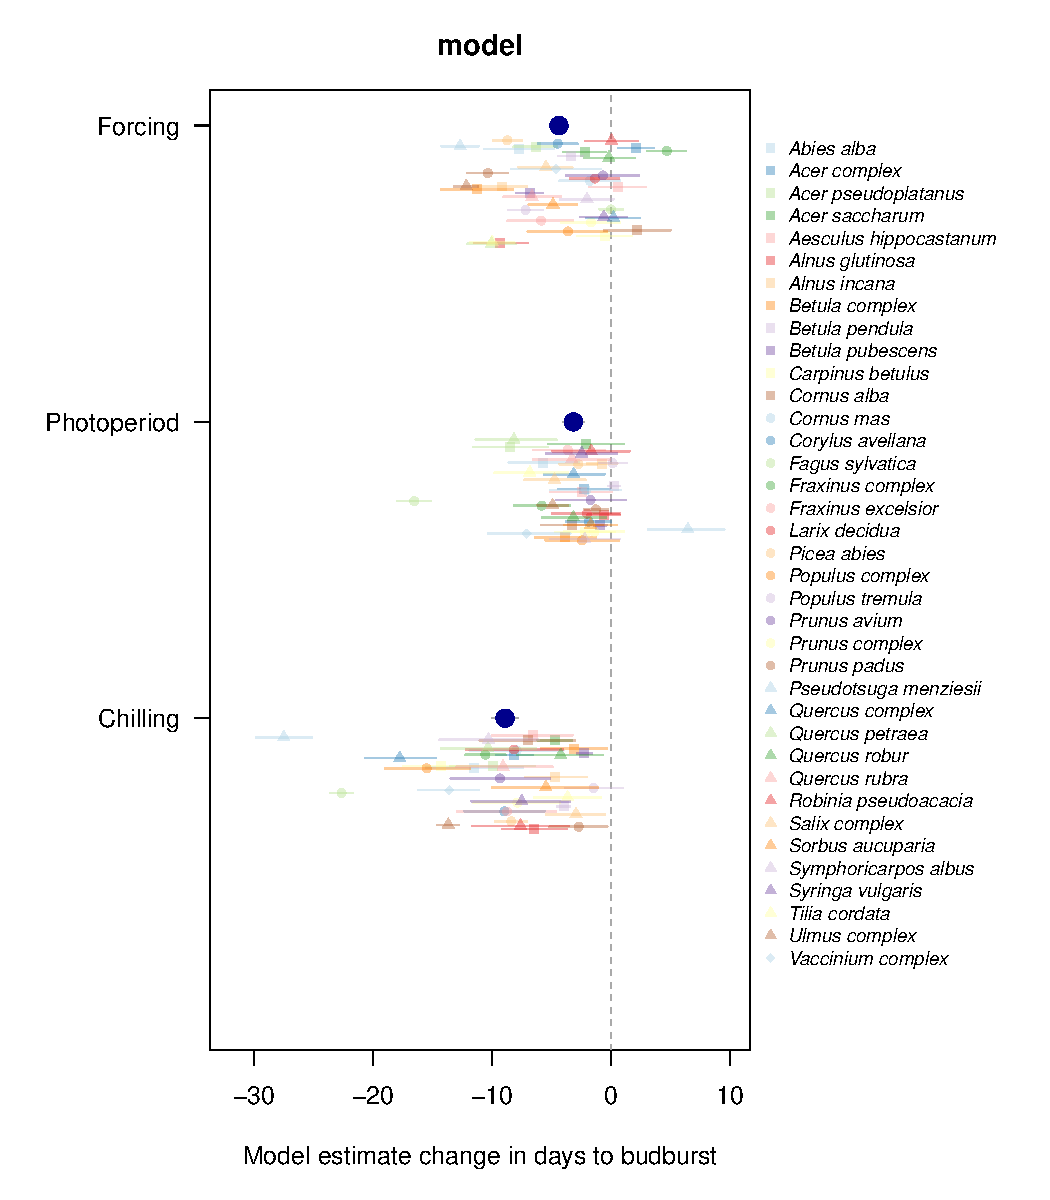
\includegraphics[width=0.75\textwidth]{..//..//analyses/bb_analysis/figures/muplotmodelspcompexprampfputah_z.pdf}
\caption{\textbf{Estimates for effects of chilling exceeded forcing and photoperiod estimates} in the budburst models fit to data from the OSPREE database. Here we show estimates from the model fit to centered data, enabling comparisons of effects sizes across predictors, and using Utah units to quantify chilling. Estimates to models fit to uncentered data and using Chill Portions were qualitatively similar and can be found in the Supplemental Materials.} 
\label{fig:mu}
\end{figure}

\newpage
\begin{figure}[h!]
\centering
\noindent 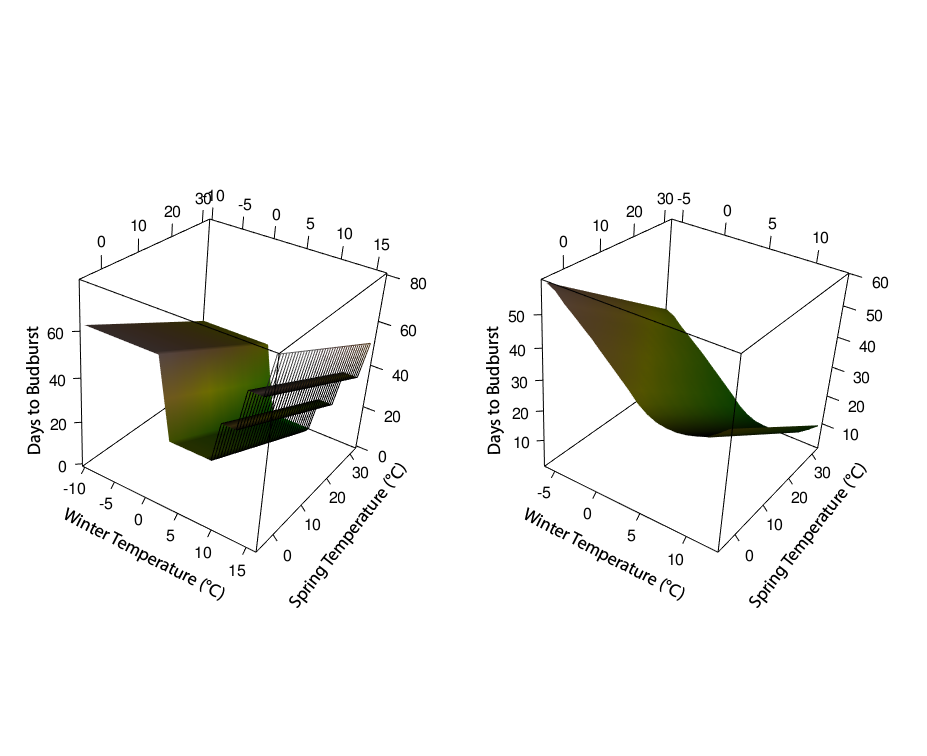
\includegraphics[width=0.75\textwidth]{..//..//analyses/bb_analysis/figures/bbmod_3dplot_utah_withPEP.png}
\caption{\textbf{Based on the OSPREE model, days to budburst decrease linearly with forcing temperature and vary nonlinearly with chilling temperature} due to the way that chilling is estimated (in this case, the Utah model; the model with Chill Portions is shown in the Supplemental Materials). Forcing treatment temperatures in growth chamber experiments ranged from 0-32 \degree C and chilling temperatures ranged from -10-16 \degree C(see Table 2S for details). Budburst responses predicted by the main budburst model are shown across the full range of experimental conditions in the OSPREE database with chilling calculated in two ways: A) as a constant temperature across a range of durations (as  is commonly applied in experiments); and B) with varying temperatures and durations using field conditions across multiple sites within the distribution of \emph{Betula pendula}, a European species that is one of the most common in OSPREE. See supplemental materials for details.}
\label{fig:apc}
\end{figure}
\newpage

\begin{figure}[h!]
\centering
\noindent 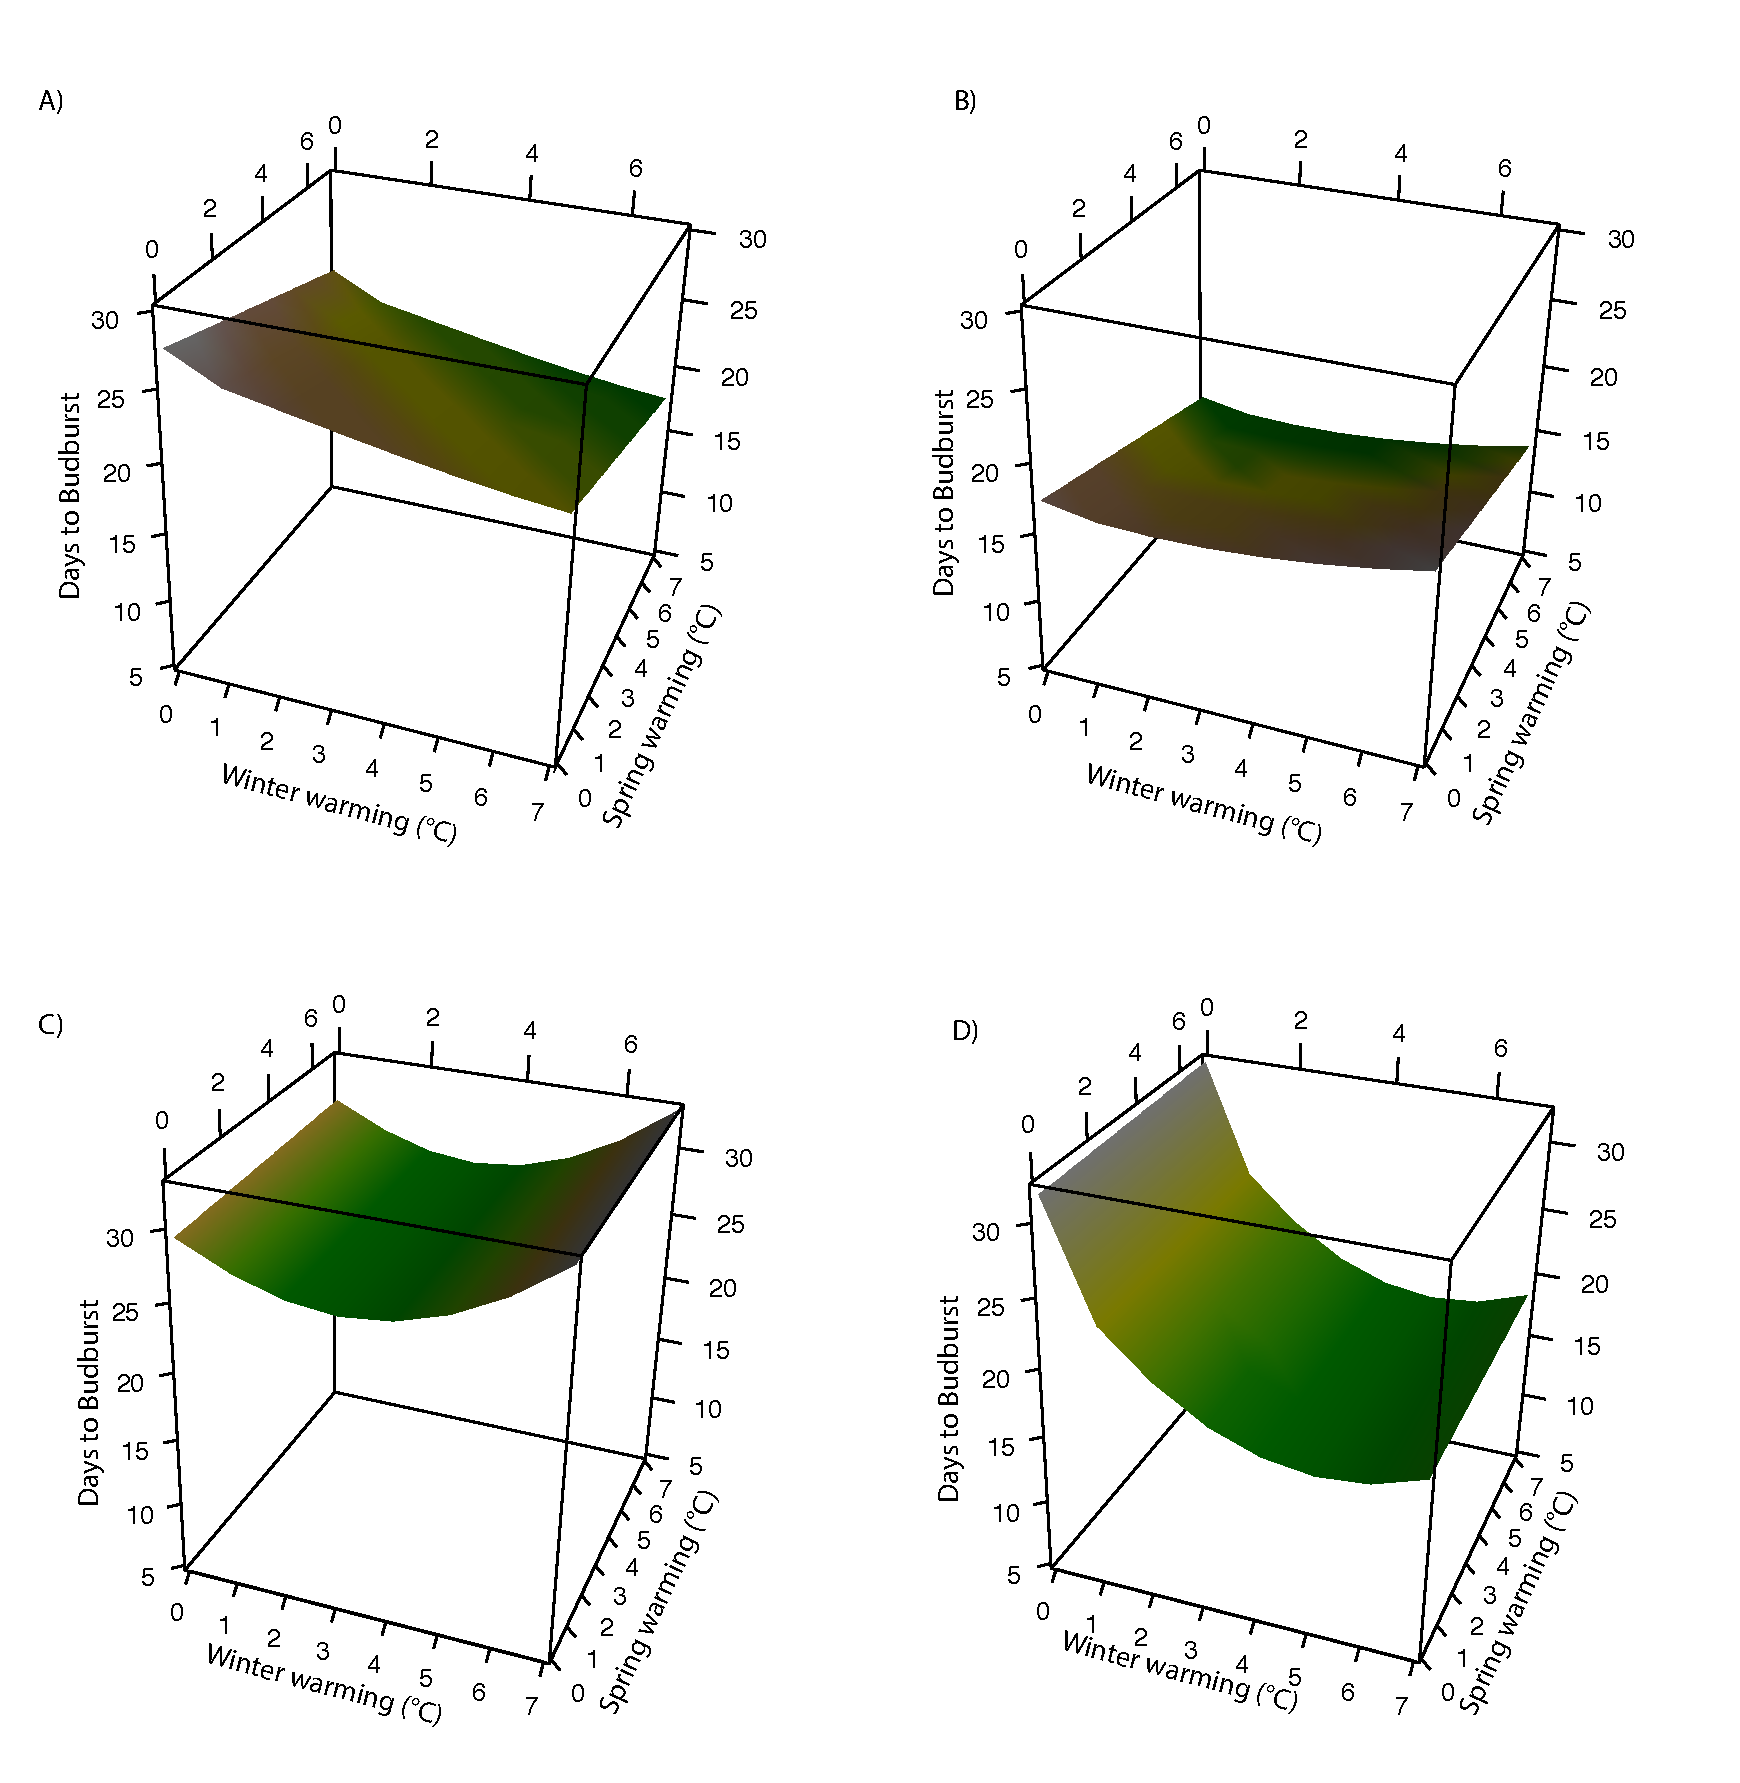
\includegraphics[width=0.75\textwidth]{..//..//analyses/bb_analysis/figures/forecasting/bbmod_3dplot_utah_obs.pdf}
\caption{\textbf{Implications of global warming on budburst varies by site}, depending on pre-warming climate for the two most common species in the OSPREE database: \emph{Betula pendula} (A,B) and \emph{Fagus sylvatica} (C,D), as predicted by the OSPREE model. For sites in A and D, chilling increases with warming, whereas chilling decreases with warming for the sites in B and C. See Supplemental Materials, especially Fig. 3S, for details.}
\label{fig:fore}
\end{figure}

%%%%%%%%%%%%%%%%%%%%%%%%%%%%%%%%%%%%%%%%
\end{document}
%%%%%%%%%%%%%%%%%%%%%%%%%%%%%%%%%%%%%%%%
